% Copyright Luke Olson 2009--2014
% This work is licensed under the Creative Commons
% Attribution-NonCommercial-NoDerivatives 4.0 International License. To view a
% copy of this license, visit http://creativecommons.org/licenses/by-nc-nd/4.0/.
%
\documentclass[10pt]{beamer}
%\documentclass[handout,10pt]{beamer}
%pdflatex -jobname lecture15.print lecture15
%
\mode<presentation>
{
  \usetheme[secheader]{Boadilla}
  \usefonttheme[onlymath]{serif}
  \setbeamercovered{invisible}
  \usecolortheme{luke}
  %\setbeamercovered{transparent}
  %
}
\mode<handout>
{
  \usetheme[secheader]{Boadilla}
  \usefonttheme[onlymath]{serif}
  \setbeamercovered{invisible}
  \usecolortheme{luke2}
  %\setbeamercovered{transparent}
}
\usepackage{pgf,pgfarrows,pgfnodes,pgfautomata,pgfheaps,pgfshade}
\usepackage{pxfonts}
\usepackage{eulervm}
\usepackage{listings}
%\usepackage{pgfpages}
%\pgfpagesuselayout{2 on 1}[letterpaper]
%
%
%%%%%%%%%%%%%%%%%%%%%%%%%%%%%%%%%%%%%%%%%%%%%%%%%%%%%%%%%%%%%%%%%%%%%%%%


%
%
%
\newcommand{\vb}{{\bf{b}}}
\newcommand{\ve}{{\bf{e}}}
\newcommand{\vg}{{\bf{g}}}
\newcommand{\vp}{{\bf{p}}}
\newcommand{\vr}{{\bf{r}}}
\newcommand{\vu}{{\bf{u}}}
\newcommand{\vx}{{\bf{x}}}
\newcommand{\vz}{{\bf{z}}}
\newcommand{\vA}{{\bf{A}}}
\newcommand{\vU}{{\bf{U}}}
\newcommand{\mO}{{\mathcal{O}}}
\newcommand{\mF}{{\mathcal{F}}}
\definecolor{mygray}{rgb}{0.95,0.95,0.95}
\lstset{
        language=matlab,
        numbers=left, numberstyle=\tiny, stepnumber=1, numbersep=5pt,
        basicstyle=\color{black}\ttfamily\small,
        commentstyle=\color{green}\ttfamily,
        keywordstyle=\color{blue}\ttfamily,
        stringstyle=\color{red}\ttfamily,
        showstringspaces=false,
        backgroundcolor=\color{mygray},
        breaklines,
}
\newcommand{\norm}[1]{{\ensuremath{{\|#1\|}}}}
\newcommand{\matdim}[2]{\ensuremath{#1\times#2}}
\newcommand{\rank}[1]{\ensuremath{\mathrm{rank}(#1)}}
\newcommand{\epsm}{\ensuremath{\varepsilon_m}}
\newcommand{\cmd}[1]{{\normalfont\ttfamily\bfseries#1}}

\author{L. Olson}
\institute[UIUC]
{Department of Computer Science\\
University of Illinois at Urbana-Champaign\\
\vspace{0.5cm}
Some slides by M. Heath
}
%%%%%%%%%%%%%%%%%%%%%%%%%%%%%%%%%%%%%%%%%%%%%%%%%%%%%%%%%%%%%%%%%%%%%%%%
\pgfdeclareimage[height=0.5cm]{university-logo}{./figs/uiuclogo}
\logo{\pgfuseimage{university-logo}}
%%%%%%%%%%%%%%%%%%%%%%%%%%%%%%%%%%%%%%%%%%%%%%%%%%%%%%%%%%%%%%%%%%%%%%%%
\title[CS 357]{Lecture 26}
\subtitle{FFT}
\date{December 3, 2009}

\begin{document}
% -------------------------------------------------
\begin{frame}
  \titlepage
\end{frame}
% -------------------------------------------------
%%%%%%%%%%%%%%%%%%%%%%%%%%%%%%%%%%%%%%%%%%%%%%%%%%%%%%%%%%%%%%%%%%%%%%%%
%%%%%%%%%%%%%%%%%%%%%%%%%%%%%%%%%%%%%%%%%%%%%%%%%%%%%%%%%%%%%%%%%%%%%%%%
\begin{frame}
\frametitle{Problem}
\begin{itemize}
\item Given some data:
  \begin{itemize}
    \item What is the nature of the data?
    \item What is the period?
    \item Can we rid the data of noise?
  \end{itemize}
\end{itemize}
\begin{center}
  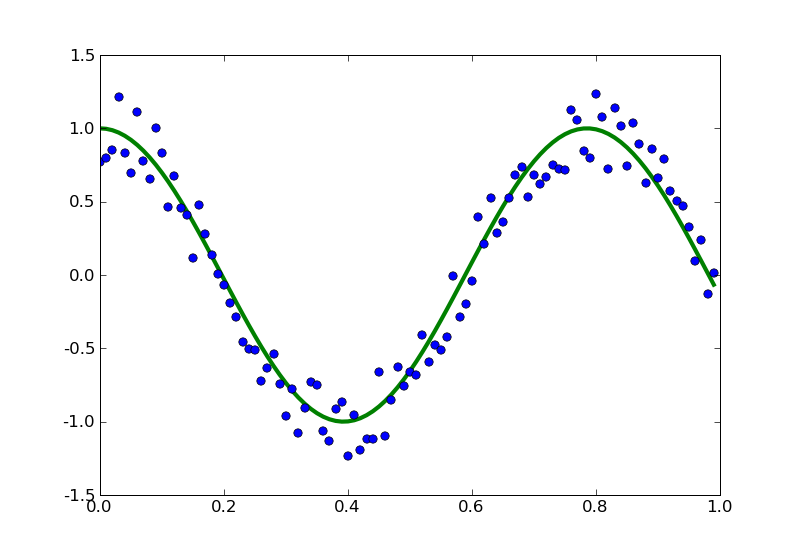
\includegraphics[width=9cm]{./figs/noisydata1}
\end{center}
\end{frame}

\begin{frame}
\frametitle{Problem}
\begin{itemize}
\item Given some data:
  \begin{itemize}
    \item What is the nature of the data?
    \item What is the period?
    \item Can we rid the data of noise?
  \end{itemize}
\end{itemize}
\begin{center}
  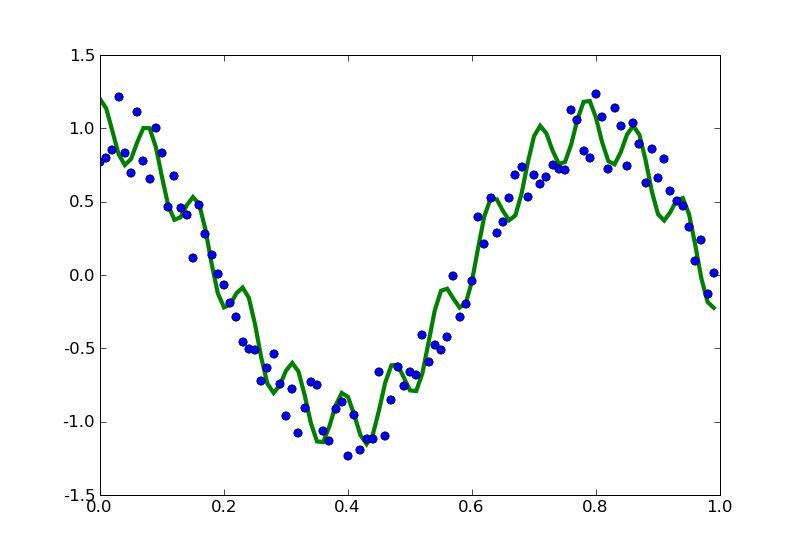
\includegraphics[width=9cm]{./figs/noisydata2}
\end{center}
\end{frame}

\begin{frame}
\frametitle{Problem}
\begin{itemize}
\item Given some data:
  \begin{itemize}
    \item What is the nature of the data?
    \item What is the period?
    \item Can we rid the data of noise?
  \end{itemize}
\end{itemize}
\begin{center}
  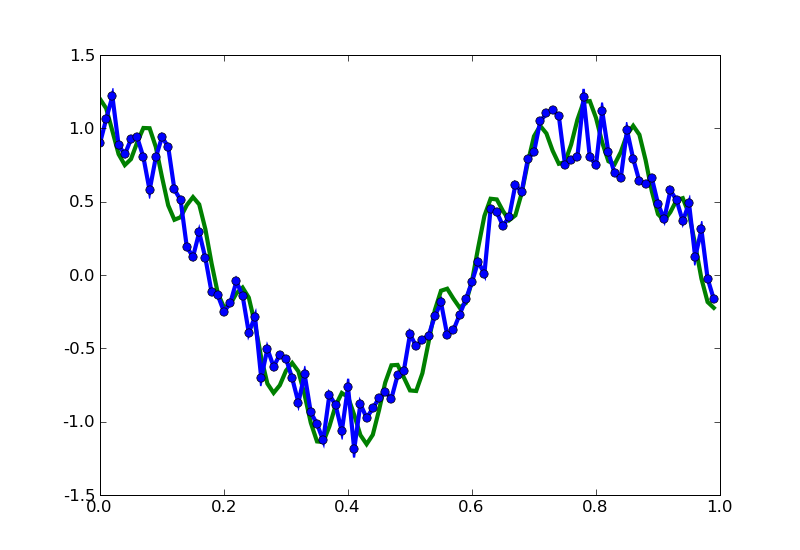
\includegraphics[width=9cm]{./figs/noisydata3}
\end{center}
\end{frame}

\begin{frame}
\frametitle{Problem Examples}
\begin{itemize}
  \item Example: remove (high-frequency) noise in an input signal
  \item Example: Weather data often contain different cycles
  \begin{itemize}
    \item daily data
    \item yearly data
    \item want to isolate one of these
  \end{itemize}
  \item Example: Economic data needs seasonal adjustment
    \begin{itemize}
    \item remove unwanted periodicities to reveal ``secular'' trends
    \end{itemize}
  \item Example: digital filtering in audio
\end{itemize}
\end{frame}
\begin{frame}
\frametitle{Problem Examples}
\begin{itemize}
  \item discrete convolution of two sequences of data $u$ and $v$ of length $n$
  \[
  \{u \star v\}_m = \sum_{k=0}^{n-1} v_k u_{m-k},\quad m = 0,1,\dots,n-1
  \]
  cross correlation of two sequences or autocorrelation with self
\end{itemize}
\begin{center}
  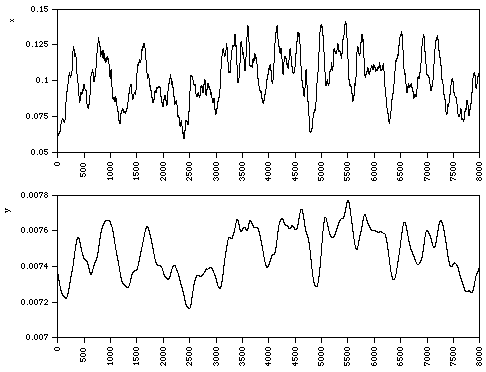
\includegraphics[width=7cm]{./figs/noisydata4}
\end{center}
\end{frame}
\begin{frame}
\frametitle{Problem Examples}
\begin{itemize}
  \item discrete convolution of two sequences of data $u$ and $v$ of length $n$
  \[
  \{u \star v\}_m = \sum_{k=0}^{n-1} v_k u_{m-k},\quad m = 0,1,\dots,n-1
  \]
  cross correlation of two sequences or autocorrelation with self
\end{itemize}
\begin{center}
  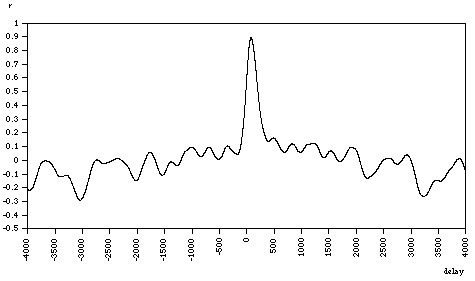
\includegraphics[width=7cm]{./figs/noisydata5}
\end{center}
\end{frame}

\begin{frame}
\frametitle{Problem Examples}
\begin{itemize}
  \item Register or align a sub image with another image:
\end{itemize}
\begin{center}
  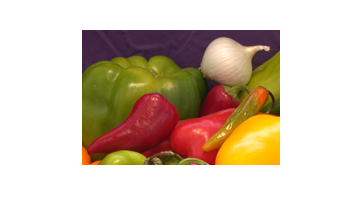
\includegraphics[width=6cm]{./figs/image_corr2}
  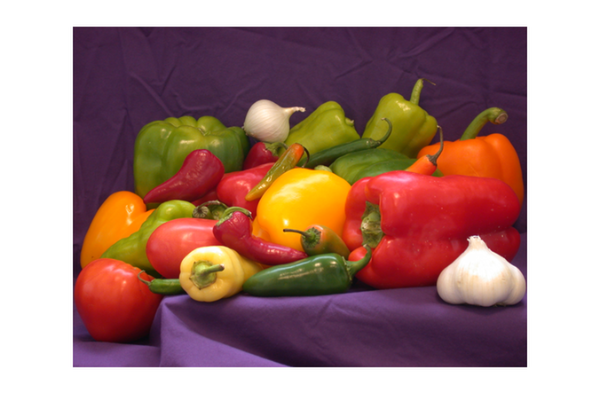
\includegraphics[width=6cm]{./figs/image_corr1}
\end{center}
\url{http://www.mathworks.com/products/image/demos.html?file=/products/demos/shipping/images/ipexnormxcorr2.html}
\end{frame}
\begin{frame}
\frametitle{Other Applications}
\begin{itemize}
  \item Spectral Analysis
  \item Data compression
  \item Partial Differential Equations
  \item Multiplication of polynomials
\end{itemize}
\end{frame}

\begin{frame}
\frametitle{Interpolation by trig}
\begin{itemize}
  \item When we have periodic data, use periodic interpolating functions: sines,
cosines, etc
\bigskip

  \item Decompose a function into a combination of sines and cosines (as we did
with polynomial basis functions)
\bigskip

  \item Decomposing into (co)sines of different ``frequencies'' naturally orders
the data.
\bigskip

  \item The gist: working in a frequency (transformed) space is easier (faster)
than the time domain.
\end{itemize}
\end{frame}

\begin{frame}
  \frametitle{Recall Fourier}
  \begin{itemize}
  \item Suppose $f(x)$ is periodic on $[-\pi,\pi]$, then the Fourier Series for
$f(x)$ is
\[
  f(x) \approx \frac{a_0}{2} + \sum_{n=1}^{\infty} a_n \cos(nx) + b_n \sin(nx)
\]
with
\[
  a_n = \frac{1}{\pi} \int_{-\pi}^{\pi} f(x) \cos(nx)\, dx \quad
  b_n = \frac{1}{\pi} \int_{-\pi}^{\pi} f(x) \sin(nx)\, dx
\]
  \item Example: $f(x) = x$ on $[-\pi,\pi]$ (sawtooth).  Then
\[
  a_n = \frac{1}{\pi} \int_{-\pi}^{\pi} x \cos(nx)\, dx  = 0
\]
\[
  b_n = \frac{1}{\pi} \int_{-\pi}^{\pi} x \sin(nx)\, dx = 2 \frac{(-1)^{n+1}}{n}
\]
so
\[
  f(x) = 2\sum_{n=1}^{\infty} \frac{(-1)^{n+1}}{n} \sin(nx)
\]
  \end{itemize}
\end{frame}
\begin{frame}
\frametitle{Sawtooth Forier}
\begin{center}
  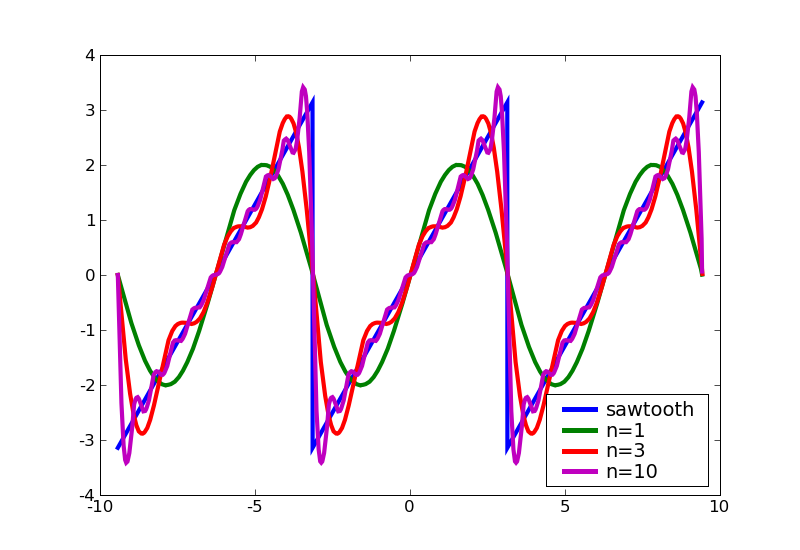
\includegraphics[width=12cm]{./figs/sawtooth}
\end{center}
\end{frame}

\begin{frame}
\frametitle{General Fourier}
\begin{itemize}
  \item Use complex exponential notation using Euler's Identity:
\[
  e^{i x} = \cos(x) + i sin(x),\qquad i = \sqrt{-1}
\]
  \item Pure cosine and sine and be written with this:
\[
  \cos(x) = \frac{e^{i x} + e^{-x}}{2},\quad \sin(x) = \frac{e^{i x} -
e^{-x}}{2i}
\]

  \item Then a Fourier Series on interval $[a,b]$ with period $\tau$ is
\[
  g(x) = \sum_{n=-\infty}^{\infty} G_n e^{i 2 \pi n x / \tau}
\]
with
\[
G_n = \frac{1}{\tau} \int_{a}^{b} g(x) e^{-i 2\pi n x / \tau}\, dx
\]
\end{itemize}
\end{frame}
\begin{frame}
\frametitle{Roots of Unity}
\begin{itemize}
  \item A primitive $n^{th}$ rooth of unity for integer $n$ is given by
\[
  \omega_n = \cos(\frac{2\pi}{n}) - i \sin(\frac{2\pi}{n}) = e^{-\frac{2\pi i}{n}}
\]
  
  \item The $n^{th}$ roots of unity are called twiddle factors here and are
given by $\omega_n^k$ or $\omega_n^{-k}$, $k=0,\dots,n-1$
\end{itemize}

demo: 
\bigskip

\url{http://www.cse.uiuc.edu/iem/fft/twdlfctr/}
\end{frame}

\begin{frame}
  \frametitle{Discrete Fourier Transforms}
  \begin{itemize}
  \item The Discrete Fourier Transform (DFT) of sequence $x =
[x_0,\dots,x_{n-1}]^T$ is a sequence $y = [y_0,\dots,y_{n-1}]^T$ given by
\[
y_m = \sum_{k=0}^{n-1} x_k \omega_n^{mk}, \quad m=0,1,\dots,n-1
\]
  \item in matrix notation this is
  \[
  y=F_n x,\qquad \{F_n\}_{mk} = \omega_n^{mk}
\]
  \item Example with $n=4$:
  \[
  F_4 = 
\begin{bmatrix}
1 & 1 & 1 & 1\\
1 & \omega^1 & \omega^2 & \omega^3\\
1 & \omega^2 & \omega^4 & \omega^6\\
1 & \omega^3 & \omega^6 & \omega^9\\
\end{bmatrix}
=
\begin{bmatrix}
1 & 1 & 1 & 1\\
1 & -i & -1 & i\\
1 & -1 & 1 & -1\\
1 & i & -1 & -i\\
\end{bmatrix}
\]
  \end{itemize}
\end{frame}

\begin{frame}
  \frametitle{Inverse Discrete Fourier Transforms}
  \begin{itemize}
  \item Note:
  \[
\frac{1}{n}
\begin{bmatrix}
1 & 1 & 1 & 1\\
1 & \omega^{-1} & \omega^{-2} & \omega^{-3}\\
1 & \omega^{-2} & \omega^{-4} & \omega^{-6}\\
1 & \omega^{-3} & \omega^{-6} & \omega^{-9}\\
\end{bmatrix}
\begin{bmatrix}
1 & 1 & 1 & 1\\
1 & \omega^1 & \omega^2 & \omega^3\\
1 & \omega^2 & \omega^4 & \omega^6\\
1 & \omega^3 & \omega^6 & \omega^9\\
\end{bmatrix}
=
\begin{bmatrix}
1 & 0 & 0 & 0\\
0 & 1 & 0 & 0\\
0 & 0 & 1 & 0\\
0 & 0 & 0 & 1\\
\end{bmatrix}
\]
  \item So $F_n^{-1} = \frac{1}{n} F_n^{*}$.
  \item Thus the Inverse DFT is
\[
x_k = \frac{1}{n} \sum_{m=0}^{n-1} y_m \omega_n^{-mk}, \quad k=0,1,\dots,n-1
\]

  \item Result: DFT, IDFT give trigonometric interpolation using only a mat-vec
$\mO(n^2)$.
  \end{itemize}
\end{frame}
\begin{frame}
\frametitle{DFTs}
  \begin{itemize}
  \item The DFT $y$ of a real sequence $x$ is generally complex
  \item Components of $y$ are then conjugate symmetric: $y_k = \bar{y}_{n-k}$,
$k=1,\dots, (n/2)-1$
  \item Two special components:
  \begin{enumerate}
  \item $y_0$ is the sum of the components of x.  This is the zero frequency
component (constant function or DC component)
  \item $y_{n/2}$ has the highest representable frequency (Nyquist frequency)
  \end{enumerate}
  \item Components beyond Nyquist are negatives of those below Nyquist.
  \end{itemize}
\end{frame}
\begin{frame}
\frametitle{Example: DFT}
\begin{itemize}
  \item For a random sequence:
\[
  y = F_8 x = F_8 
  \begin{bmatrix}
4\\ 0\\ 3\\ 6\\ 2\\ 9\\ 6\\ 5\\
  \end{bmatrix}
  \begin{bmatrix}
  35.0          \\
  -5.1 + 8.7i\\
  -3.0 + 2.0i\\
   9.1 + 2.7i\\
  -5.0          \\
   9.1 - 2.7i\\
  -3.0 - 2.0i\\
  -5.1 - 8.7i\\
  \end{bmatrix}
\]
\item The transformed sequence is complex, but $y_0$ and $y_4$ are real, while
$y_5$, $y_6$, and $y_7$ are complex conjugates of $y_3$, $y_2$, and $y_1$,
respectively.
\item $y_0$ is in fact the sum
\end{itemize}
\end{frame}
\begin{frame}
\frametitle{Example: DFT}
\begin{itemize}
  \item For a cyclic sequence:
\[
  y = F_8 x = F_8 
  \begin{bmatrix}
1\\ -1\\
1\\ -1\\
1\\ -1\\
1\\ -1\\
  \end{bmatrix}
  \begin{bmatrix}
0\\ 0\\
0\\ 0\\
8\\ 0\\
0\\ 0\\
  \end{bmatrix}
\]
\item Sequence $x$ has highest rate of oscillation possible for this sample.
\item Sequence $y$ has only nonzero component at the Nyquist frequency
\item \url{http://www.cse.uiuc.edu/iem/fft/dgtlfltr/}
\end{itemize}
\end{frame}
\begin{frame}
\frametitle{Computing the DFT}
\begin{itemize}
  \item Goal: take advantage of symmetries in the DFT for efficiency
  \item Consider $n=4$:
\[
y_m = \sum_{k=0}^3 x_k \omega_n^{mk}, \quad m=0,\dots,3
\]
or
\begin{align*}
  y_0 & = x_0 \omega_n^0 + x_1 \omega_n^0 + x_2 \omega_n^0 + x_3 \omega_n^0\\
  y_1 & = x_0 \omega_n^0 + x_1 \omega_n^1 + x_2 \omega_n^2 + x_3 \omega_n^3\\
  y_2 & = x_0 \omega_n^0 + x_1 \omega_n^2 + x_2 \omega_n^4 + x_3 \omega_n^6\\
  y_3 & = x_0 \omega_n^0 + x_1 \omega_n^3 + x_2 \omega_n^6 + x_3 \omega_n^9\\
\end{align*}
\end{itemize}
\end{frame}
\begin{frame}
\frametitle{Computing the DFT}
\begin{itemize}
  \item $\omega_n^0=\omega_n^4 = 1$, $\omega_n^2=\omega_n^6 = -1$,
$\omega_n^9=\omega_n^1$ so
\begin{align*}
  y_0 & = (x_0 + x_2 \omega_n^0) + \omega_n^0 (x_1 + \omega_n^0 x_3)\\
  y_1 & = (x_0 - x_2 \omega_n^0) + \omega_n^1 (x_1 - \omega_n^0 x_3)\\
  y_2 & = (x_0 + x_2 \omega_n^0) + \omega_n^2 (x_1 + \omega_n^0 x_3)\\
  y_3 & = (x_0 - x_2 \omega_n^0) + \omega_n^3 (x_1 - \omega_n^0 x_3)\\
\end{align*}
  \item some of these are $1$ ($\omega_n^0$), but even so we have 8 additions
and 6 multiplications
  \item without the simplification this is 12 additions, 16 multiplications
\end{itemize}
\end{frame}
\begin{frame}
\frametitle{Computing the DFT}
\begin{itemize}
  \item Computing the DFT of the 4 point problem reduced to computing the DFT of
its two 2 point even and odd subsequences.

\item Generally, the pattern emerges
\[
F_1 = 1,\quad
F_2 = \begin{bmatrix}1 & 1\\ 1& -1\\\end{bmatrix},\quad
F_4 = 
\begin{bmatrix}
1 & 1 & 1 & 1\\
1 & -i & -1 & i\\
1 & -1 & 1 & -1\\
1 & i & -1 & -i\\
\end{bmatrix}
,\dots
\]
\end{itemize}
\begin{alertblock}{}
The DFT of an $n-$point sequence can be computing by two $n/2$-point DFTS ($n$
even)
\end{alertblock}
\end{frame}
\begin{frame}
\frametitle{Computing the DFT}
\begin{itemize}
  \item Let $P_4$ be a permulation matrix
\[
  P_4 =
\begin{bmatrix}
1 & 0 & 0 & 0\\
0 & 0 & 1 & 0\\
0 & 1 & 0 & 0\\
0 & 0 & 0 & i\\
\end{bmatrix}
\]
and $D_2$ be the diagonal matrix
\[
  D_2 = 
\begin{bmatrix}
1 & 0\\ 0 & \omega_4 = -i\\
\end{bmatrix}
\]

\item Then
\[
  F_4 P_4 =
\begin{bmatrix}
1 & 1 & 1 & 1\\
1 & -1 & -i & i\\
0 & 1 & -1 & -1\\
1 & -1 & i & -i\\
\end{bmatrix}
=
\begin{bmatrix}
F_2 & D_2 F_2\\
F_2 & -D_2 F_2\\
\end{bmatrix}
\]

\end{itemize}
\end{frame}
\begin{frame}
\frametitle{Computing the DFT}
\framesubtitle{from M. Heath}
\begin{itemize}
  \item So $F_4$ can be rearranged to diagonally scaled blocks of $F_2$
  \item Holds for any even $n$
  \item In general, $P_n$ is a permutation that groups even numbered columns
then odd numbered columns.  And $D_{n/2} =
diag(1,\omega_n,\dots,\omega_n^{(n/2)-1}$.
  \item To apply $F_n$, apply $F_{n/2}$ to the even and odd subsequences and
scale the results (where necessary) by $\pm D_{n/2}$.
  \item This recursive $DFT$ is called the Fast Fourier Transform (FFT)
\end{itemize}
\end{frame}
\begin{frame}
\frametitle{FFT}
\begin{center}
  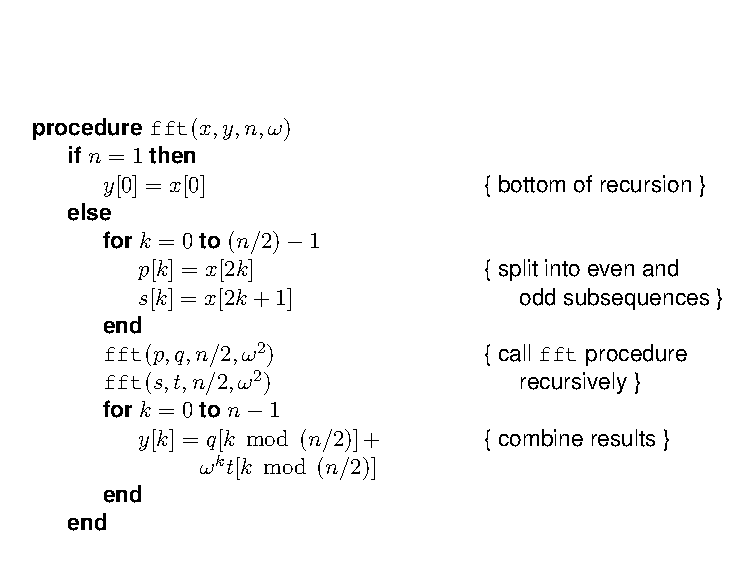
\includegraphics[width=\textwidth]{./figs/fft_alg}
\end{center}
\end{frame}
\begin{frame}
\frametitle{FFT}
\begin{itemize}
  \item Cost: $\log_2 n$ levels of recursion, with $\mO(n)$ operations each.  So
a total cost of $\mO(n\log_2 n)$.
  \item Often the transform is computed in-place in one array
  \item More reductions (storage and operation count in half) if $x$ is real
  \item Final sequence $y$ can be ordered in $\mO(n \log_2 n)$ by a sort
  \item Can write as iteration rather than recursion.
  \item Still an {{\underline{algorithm}}}: one particular way of computing the
DFT
  \item \url{http://www.cse.uiuc.edu/iem/fft/rcrsvfft/}
\end{itemize}
\end{frame}
\end{document}
